\section{Ход выполнения работы}

\subsection{Исходная модель и средства выполнения}

Исходный проект \path{ARIA-StarUML2.mdj} содержит модель анализа ARIA,
диаграммы прецедентов, классов, последовательностей, деятельности и пакетов.
В рабочую модель \path{lab6/ARIA-Lab6.mdj} добавлен пакет
«06. Проектирование и инженерия». Исходные 21 диаграмма сохранены.

Для трассировок выбраны классы из пакета
«21. Распределение классов с интерфейсами». В нём находятся 28 классов:
11 граничных, 7 управляющих и 10 сущностей. Это один согласованный срез
модели; копии классов на других диаграммах исходного проекта отдельно
не трактуются как новые предметные сущности.

В исходной модели язык программирования и СУБД не заданы.
Для лабораторной приняты Python 3 и PostgreSQL: аннотации Python
позволяют явно описать параметры, а PostgreSQL поддерживает UUID,
JSONB и отложенные внешние ключи. Эти технологии являются решениями
данной работы, а не установленными свойствами исходного проекта.
Типы указаны непосредственно в UML-атрибутах и параметрах;
профиль языка Enterprise Architect в StarUML не создавался.

Все новые элементы и представления созданы внутри StarUML 7.1.1
вызовами \texttt{Factory} и \texttt{Engine}. Модель сохранена
его \texttt{ProjectManager}; SVG-диаграммы и документация получены
его экспортерами. Для отчёта SVG преобразованы в векторные PDF
и растровые PNG: это устраняет дефект рамок штатного PNG-экспорта,
не изменяя элементы и расположение диаграмм.
Сценарии \path{scripts/lab6-model.cjs}
и \path{scripts/lab6-finish.cjs} запускаются встроенной командой EJS.
Диаграммы в сторонних графических редакторах не строились.

\clearpage
\subsection{Трассировка граничных классов}

Восемь граничных классов экранов сопоставлены классам форм:
анализа аудиозаписи, анализа каталога, поиска, активных заданий,
истории, результата, параметров и входа.
Ещё три границы сопоставлены входному адаптеру Catalog Service,
клиенту Auth Service и адаптеру файлового хранилища.
Таким образом, покрыты все 11 граничных классов выбранного среза.

На диаграммах связи \texttt{\guillemotleft trace\guillemotright}
направлены от элемента анализа к его проектной реализации.
Формы имеют закрытый атрибут \texttt{service} с типом соответствующего
сервиса и открытую операцию
\texttt{handle(payload: dict[str, str]): dict[str, str]}.
Контракт описывает передачу полей формы; реализация интерфейса
и обработчиков в состав учебного каркаса не входит.

\labDiagram{22}{Трассировка граничных классов в классы форм}{fig:boundary-forms}
\labInlineDiagram{23}{Трассировка интеграционных границ в адаптеры}{fig:boundary-adapters}

Catalog Service и Auth Service сохраняют статус внешних систем.
Внутри ARIA находятся только их адаптеры. \texttt{AuthClient}
передаёт проверку учётных данных внешней системе;
локальная БД ARIA не содержит паролей.

\subsection{Управляющие классы и классы проектирования}

Каждый из семи управляющих классов получил проектную реализацию
в соответствующей подсистеме (рисунок~\ref{fig:control-trace}).
Имена методов Python связаны с операциями исходных классов:
например, «Найти аудиозаписи» соответствует \texttt{search},
«Создать задание» --- \texttt{create},
«Установить пороги» --- \texttt{set\_thresholds}.

\labDiagram{24}{Трассировка управляющих классов}{fig:control-trace}

\texttt{AudioAnalysisService} запускает анализ, получает аудиофайл,
определяет характеристики и отбирает оценки по порогам.
Закрытые атрибуты: \texttt{model\_name: str} и
\texttt{thresholds: dict[str, float]}. Открытая операция
\texttt{start(audio\_id: UUID): UUID} возвращает идентификатор задания;
\texttt{get\_audio\_file(audio\_id: UUID): bytes} --- содержимое файла.
\texttt{extract\_features(audio: bytes): dict[str, float]} и
\texttt{filter\_scores(scores: dict[str, float]): dict[str, float]}
возвращают характеристики и принятые оценки соответственно.

\texttt{CatalogAnalysisService} реализует повторный анализ каталога.
Закрытые атрибуты: \texttt{filters: dict[str, str]} и
\texttt{scheduled\_at: datetime | None}.
\texttt{start\_catalog(filters, scheduled\_at): list[UUID]}
возвращает идентификаторы заданий;
\texttt{select\_audio(filters): list[UUID]} --- выбранные аудиозаписи.
Тип параметра \texttt{filters} в обеих операциях ---
\texttt{dict[str, str]}, времени --- \texttt{datetime | None}.

\texttt{AudioSearchService} содержит закрытые
\texttt{description: str} и \texttt{filters: dict[str, str]}.
Операция \texttt{search(description: str, filters: dict[str, str]): list[UUID]}
возвращает найденные аудиозаписи;
\texttt{build\_conditions(): dict[str, str]} формирует условия поиска.

\labDiagram{26}{Атрибуты и операции сервисов анализа и поиска}{fig:design-search}

\texttt{AnalysisJobService} хранит
\texttt{current\_job\_id: UUID | None}.
Его операции: \texttt{create(audio\_id: UUID): UUID},
\texttt{save\_result(job\_id: UUID, scores: dict[str, float]): None},
\texttt{list\_jobs(): list[UUID]},
\texttt{cancel(job\_id: UUID): bool} и
\texttt{get\_status(job\_id: UUID): str}.
Они соответствуют созданию задания, сохранению результата,
просмотру заданий, отмене и получению статуса.

\texttt{AnalysisResultService} имеет закрытый
\texttt{export\_format: str}. Операции предоставляют историю, результат,
удаление и выгрузку:
\begin{flushleft}\small\ttfamily
get\_history(): list[UUID]\\
get\_result(job\_id: UUID): dict[str, float]\\
delete\_result(job\_id: UUID): bool\\
export\_history(): bytes
\end{flushleft}
Формат экспорта в исходной модели --- Parquet.

\texttt{AnalysisSettingsService} хранит закрытые
\texttt{model\_name: str}, \texttt{weights\_path: str} и
\texttt{thresholds: dict[str, float]}.
Операции \texttt{select\_model(name: str): None},
\texttt{import\_model(file: str, name: str): None} и
\texttt{set\_thresholds(thresholds: dict[str, float]): None}
соответствуют выбору модели, импорту весов и изменению порогов.

\texttt{AuthServiceAdapter} реализует управляющий класс «Вход в систему».
Закрытый атрибут --- \texttt{principal\_id: UUID | None}.
Операции: \texttt{login(login: str, password: str): UUID},
\texttt{get\_permissions(): list[str]} и
\texttt{check\_permission(action: str): bool}.
Все описанные методы сервисов открытые; знак «$-$» на диаграммах
обозначает закрытые атрибуты, «$+$» --- открытые операции.

\labDiagram{27}{Атрибуты и операции остальных сервисов}{fig:design-other}

\subsection{Пакеты анализа и подсистемы}

Восемь пакетов анализа сопоставлены восьми \texttt{UMLSubsystem}
с теми же названиями. Проектные классы размещены в подсистемах
по ответственности. Пакет «Аудиозаписи» соответствует подсистеме
доступа к метаданным; её хранимые структуры раскрыты моделями БД.

Анализ использует задания, параметры, аудиозаписи и файловое хранилище;
поиск использует аудиозаписи. Входной интерфейс Catalog Service
обращается к анализу и заданиям.
Интеграционные подсистемы не представляют сами внешние сервисы.

\labDiagram{25}{Трассировка пакетов анализа в подсистемы}{fig:package-trace}
\labDiagram{36}{Зависимости подсистем ARIA}{fig:subsystem-dependencies}

\subsection{Прямое и обратное проектирование}

Из UML-атрибутов и операций семи сервисов встроенной командой EJS
StarUML с пользовательским шаблоном получен файл
\path{lab6/generated/aria_design.py}.
Закрытым атрибутам соответствует префикс \texttt{\_}; типы,
параметры и возвращаемые значения перенесены в аннотации Python.
Методы содержат \texttt{raise NotImplementedError}:
генерация создаёт структурный каркас, а не действующий сервис анализа.

Для обратного проектирования подготовлена отдельная копия:
\path{lab6/reverse-input/aria_design.py}.
В ней класс \texttt{AudioSearchService} изменён следующим образом:
\begin{enumerate}
  \item Добавлен закрытый атрибут \texttt{\_limit: int}.
  \item Добавлена открытая операция \texttt{set\_limit(limit: int): None}.
  \item В \texttt{search} добавлен параметр \texttt{limit: int}.
  \item Удалена операция \texttt{build\_conditions}.
\end{enumerate}

Скрипт \path{scripts/reverse_python.py} разобрал реальный изменённый
файл модулем \texttt{ast}. Полученные классы, атрибуты и сигнатуры
импортированы сценарием StarUML в отдельный пакет
«04. Обратное проектирование Python». Это структурный импорт,
а не обновление исходных классов на месте. Его результат сравнен
с AST: совпадение подтверждено в
\path{lab6/validation/reverse-import.json}.
Обе версии Python-кода успешно компилируются. Перечень изменений
сохранён в \path{lab6/roundtrip-changes.json}, текстовое сравнение ---
в \path{lab6/roundtrip.diff}.

\labDiagram{38}{Сопоставление исходного и восстановленного класса поиска}{fig:reverse-search}

\subsection{Инфологическая модель и трассировка сущностей}

В инфологической модели уточнены все 10 сущностей выбранного среза
анализа. Основу составляют «Аудиозапись», «Файл», «Тег» и
«Эмоциональная метка». Аудиозапись связана с файлом отношением 1:1,
а с тегами и эмоциональными метками --- M:N с необязательным участием.
Название и автор являются локальными метаданными для анализа и поиска;
исходный каталог остаётся внешним Catalog Service.

Служебная часть включает пользователя, задание анализа, оценку
уверенности, модель, профиль весов и порог уверенности.
Пользователь --- локальная проекция идентификатора и имени из Auth Service.
Задание связано с аудиозаписью и моделью, содержит снимок порогов
при запуске и набор оценок. У модели один профиль весов и множество
порогов. Связи не вводят новых прецедентов.

Технический ключ \texttt{id: UUID} добавлен при проектировании хранения.
Темп измеряется в ударах в минуту, длительность --- в секундах,
детюн --- в центах; тоника кодируется числом от 0 до 11.
Оценки уверенности, пороги и прогресс задаются числами от 0 до 1.
Диаграммы используют UML-классы со стереотипом \texttt{entity};
ограничения хранения раскрываются в даталогической модели и DDL.

\labDiagram{28}{Инфологическая модель аудиозаписей}{fig:logical-audio}
\labDiagram{29}{Инфологическая модель заданий и оценок}{fig:logical-analysis}
\labDiagram{39}{Инфологическая модель моделей, весов и порогов}{fig:logical-settings}
\labDiagram{32}{Трассировка классов-сущностей анализа}{fig:entity-trace}

\subsection{Даталогическая модель}

Для PostgreSQL созданы 12 ER-сущностей, представляющих таблицы.
Десять из них соответствуют сущностям инфологической модели;
\texttt{audio\_recording\_tag} и
\texttt{audio\_recording\_emotion} раскрывают связи M:N.
В связующих таблицах составной первичный ключ состоит из двух
внешних ключей. Связующие таблицы не являются новыми предметными сущностями.

Для столбцов заданы тип, длина или точность, признаки PK, FK,
UNIQUE и NULL; внешние ключи ссылаются на конкретные ER-столбцы
через свойство \texttt{referenceTo}.
Характеристики, которые ещё не определены анализом, допускают NULL.
Модель, веса и пороги связаны внешними ключами;
оценки уверенности принадлежат заданию анализа.

Сопоставление концептуальных сущностей и таблиц сохранено отдельной
диаграммой (рисунок~\ref{fig:entity-table}). В StarUML
нет применённой штатной трансформации Enterprise Architect:
правила соответствия и раскрытия M:N заданы в пользовательском сценарии.

\labDiagram{30}{Таблицы аудиозаписей, файлов и меток}{fig:physical-audio}
\labDiagram{31}{Таблицы моделей, весов и порогов}{fig:physical-settings}
\labDiagram{37}{Таблицы заданий и оценок уверенности}{fig:physical-jobs}
\labDiagram{33}{Трассировка инфологических сущностей в таблицы}{fig:entity-table}

\subsection{DDL-сценарий и проверка ограничений}

Файл \path{lab6/sql/aria.sql} сформирован в StarUML из ER-таблиц
и их столбцов пользовательским генератором.
Дополнительные CHECK, составные UNIQUE, индексы и отложенные
внешние ключи заданы явно в сценарии, поскольку они не полностью
представлены свойствами \texttt{ERDColumn}.
Таким образом, DDL не является результатом встроенной команды
генерации SQL Enterprise Architect.

Сначала создаются независимые таблицы, затем зависимые.
После создания всех таблиц добавляются два обратных отложенных
ключа: аудиозапись обязана иметь файл, а модель --- профиль весов.
Совместно с UNIQUE на \texttt{audio\_id} и \texttt{model\_id}
они обеспечивают обязательные связи 1:1 на момент завершения транзакции.
При вставке пары объектов используется одна транзакция.
На ER-диаграмме непосредственный FK показывает 0..1 со стороны
зависимой строки; обязательность завершённой пары дополнительно
задана отложенным ограничением и описана в свойствах таблицы.

Проверки ограничивают положительные темп и длительность,
диапазоны тоники, прогресса и уверенности, допустимые статусы
и порядок временных отметок. Завершённый статус требует времени
завершения. Удаление используемой модели запрещено RESTRICT;
для зависимых строк применено каскадное удаление.

Сценарий выполнен в новом изолированном кластере PostgreSQL 18.1.
Проверены создание 12 таблиц, корректные вставки и соединение
аудиозаписи с файлом и тегом, завершение задания, каскадное удаление
и обязательные связи 1:1. Восемнадцать негативных проверок получили
ожидаемые SQLSTATE: нарушение уникальности, внешних ключей,
CHECK и RESTRICT. Существующие базы пользователя не использовались;
тестовый сервер после проверки остановлен.
Результаты сохранены в \path{lab6/validation/postgresql.json}
и \path{lab6/validation/postgresql.log}.

Полный DDL приведён в приложении~А.

\subsection{Документация и проверка модели}

Штатным расширением HTML Export StarUML сгенерирован каталог
\path{lab6/docs/html/}. Файл \texttt{index.html} открывает дерево
модели, описания элементов, их свойства и диаграммы.
На рисунке~\ref{fig:docs} приведён пример страницы класса поиска.

\begin{figure}[H]
  \centering
  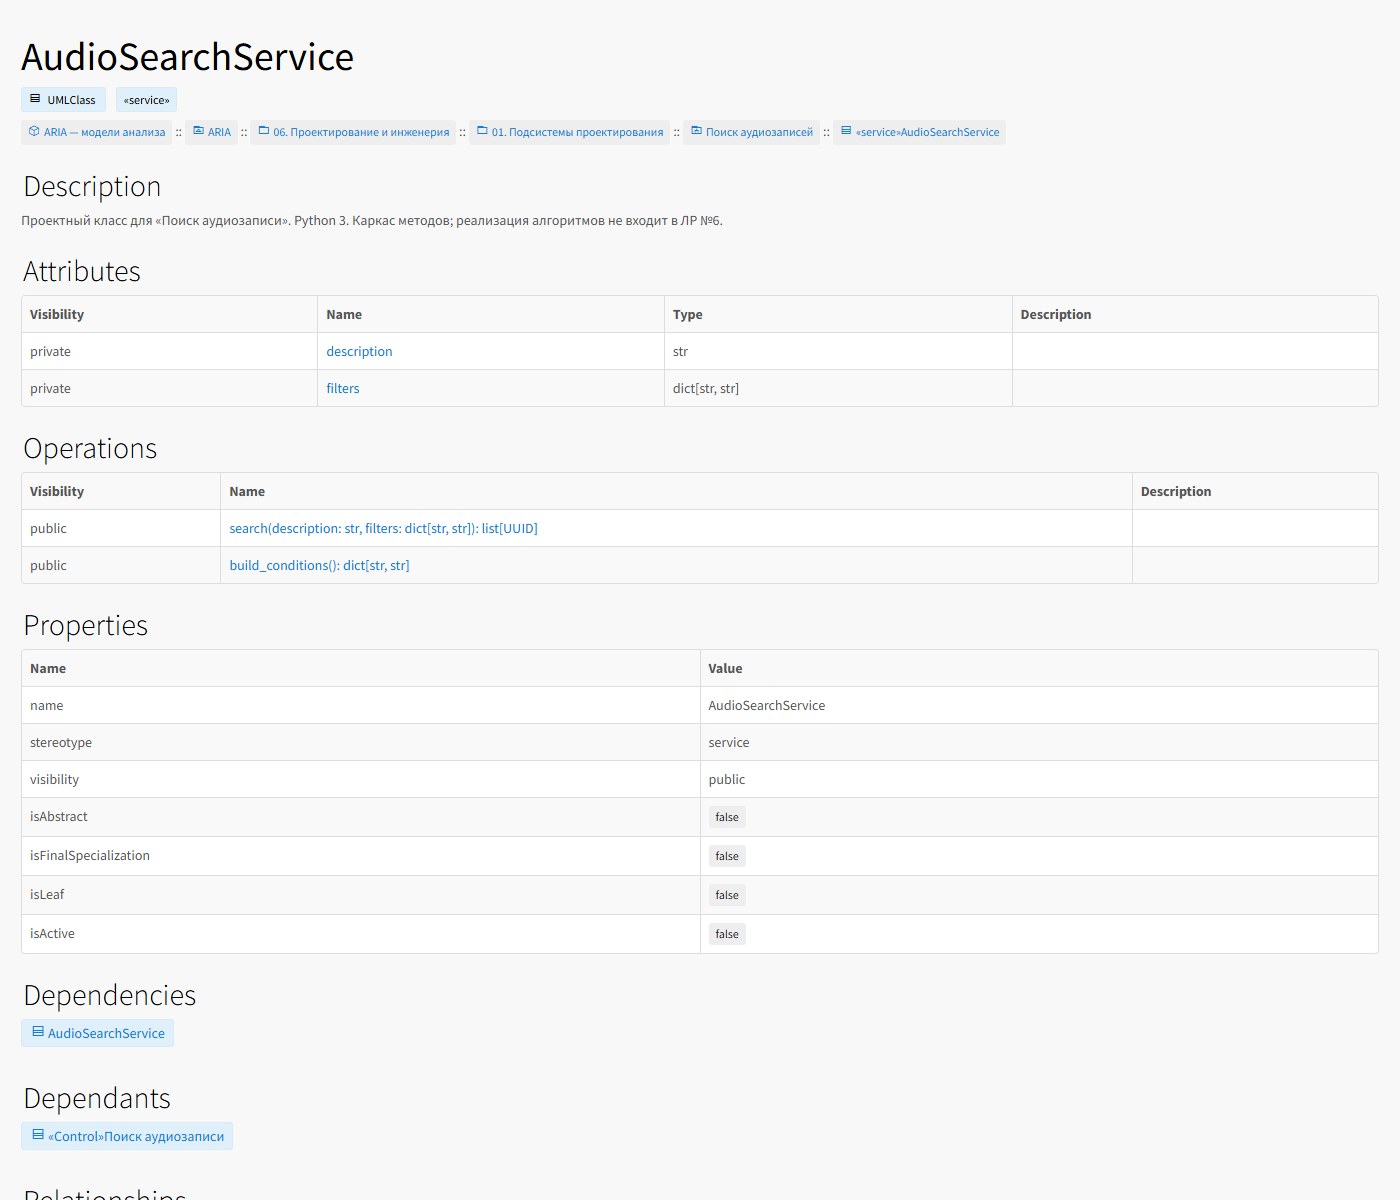
\includegraphics[width=\textwidth]{lab6/docs/documentation-example.png}
  \caption{Пример HTML-документации, сгенерированной StarUML}
  \label{fig:docs}
\end{figure}

Вызов встроенного валидатора \texttt{app.validator.validate()}
завершился без ошибок. Сохранённый результат:
\begin{Verbatim}[fontsize=\small,frame=single]
tool: StarUML 7.1.1
method: app.validator.validate()
errors: []
sourceErrors: []
lab6Errors: []
\end{Verbatim}

Это UML-валидация StarUML. Проверка целостности репозитория
Enterprise Architect не выполнялась. Дополнительно проверены
уникальность идентификаторов MDJ, разрешимость ссылок,
сохранение исходных элементов и диаграмм, наличие экспортов,
соответствие обратного импорта Python и выполнение SQL.
Результат находится в \path{lab6/validation/artifact-audit.json}.

\subsection{Статистика проекта}

Подсчёт выполнен по сохранённому MDJ-файлу, а не по числу
изображений или повторных представлений классов.
Пакеты и подсистемы учитываются раздельно.
Столбец «Вся модель» включает исходные копии классов
в разных пакетах, 18 новых классов проектирования,
10 инфологических сущностей и 7 классов обратного импорта.

\newcommand{\statSourcePackages}{43}
\newcommand{\statSourceSubsystems}{0}
\newcommand{\statSourceDiagrams}{21}
\newcommand{\statSourceUmlClasses}{140}
\newcommand{\statSourceRelationships}{368}
\newcommand{\statSourceLogicalEntities}{0}
\newcommand{\statSourceTables}{0}
\newcommand{\statTotalPackages}{51}
\newcommand{\statTotalSubsystems}{8}
\newcommand{\statTotalDiagrams}{39}
\newcommand{\statTotalUmlClasses}{175}
\newcommand{\statTotalRelationships}{446}
\newcommand{\statTotalLogicalEntities}{10}
\newcommand{\statTotalTables}{12}
\newcommand{\statLabSixPackages}{8}
\newcommand{\statLabSixSubsystems}{8}
\newcommand{\statLabSixDiagrams}{18}
\newcommand{\statLabSixUmlClasses}{35}
\newcommand{\statLabSixRelationships}{78}
\newcommand{\statLabSixLogicalEntities}{10}
\newcommand{\statLabSixTables}{12}

\begin{table}[H]
  \centering
  \caption{Статистика сохранённой модели}
  \begin{tabularx}{\textwidth}{|X|r|r|r|}\hline
    Показатель & Исходник & ЛР №6 & Вся модель \\\hline
    Пакеты UML & \statSourcePackages & \statLabSixPackages & \statTotalPackages \\\hline
    Подсистемы UML & \statSourceSubsystems & \statLabSixSubsystems & \statTotalSubsystems \\\hline
    Диаграммы & \statSourceDiagrams & \statLabSixDiagrams & \statTotalDiagrams \\\hline
    Классы UML & \statSourceUmlClasses & \statLabSixUmlClasses & \statTotalUmlClasses \\\hline
    Связи модели & \statSourceRelationships & \statLabSixRelationships & \statTotalRelationships \\\hline
    Инфологические сущности & 0 & 10 & 10 \\\hline
    ER-таблицы & 0 & 12 & 12 \\\hline
  \end{tabularx}
\end{table}

Полный машинно-читаемый результат и перечень диаграмм сохранены
в \path{lab6/statistics.json}. Связями считаются UML-ассоциации,
зависимости, потоки, сообщения, связи прецедентов и ER-связи;
концы связей и графические представления повторно не учитываются.

\subsection{Структура проекта базы данных}

Пакет «03. Проект базы данных» содержит инфологическую модель,
даталогическую модель PostgreSQL и физическую структуру хранения.
Шаблон сформирован вручную через API StarUML;
готовый шаблон Database Builder Enterprise Architect не применялся.
Трассировки сущностей и таблиц находятся в соседнем пакете
«02. Трассировка», чтобы не дублировать элементы.

PostgreSQL хранит метаданные, связи и результаты анализа;
аудиофайлы и веса моделей размещаются в файловом хранилище,
а в БД сохраняются их расположения.
Диаграмма физической структуры отражает эти роли без фиксации
неподтверждённых адресов серверов и параметров развёртывания.

\labDiagram{34}{Физическая структура хранения ARIA}{fig:deployment}
\labDiagram{35}{Структура проекта базы данных}{fig:database-structure}

\subsection{Состав результатов и особенности выполнения}

Основные результаты находятся в каталоге \path{lab6/}:
модель \texttt{ARIA-Lab6.mdj}; исходная копия в \texttt{source/};
18 диаграмм в SVG, PNG и PDF в \texttt{diagrams/};
сгенерированный и изменённый код в \texttt{generated/}
и \texttt{reverse-input/}; SQL в \texttt{sql/};
HTML-документация в \texttt{docs/html/};
проверки в \texttt{validation/}; статистика и сведения
о воспроизведении в \texttt{statistics.json} и \texttt{report.md}.
Основной отчёт подготовлен в LaTeX: \texttt{main.tex}.

Вручную спроектированы соответствия классов и подсистем,
правила преобразования сущностей, ограничения и структура БД.
Их создание автоматизировано пользовательским сценарием StarUML.
Прямое проектирование выполнено генератором EJS с пользовательским
шаблоном; обратное --- разбором AST и пользовательским импортом
в отдельный пакет. Штатная двусторонняя синхронизация Python,
автоматическая трансформация моделей БД, SQL-генератор
и проверка репозитория Enterprise Architect в данной работе
не использовались. HTML-документация, экспорт диаграмм
и UML-валидация выполнены штатными средствами StarUML.
